\documentclass[tikz, border=10pt]{standalone}
\usetikzlibrary{shapes.geometric, arrows, positioning, fit, calc, backgrounds}

\begin{document}

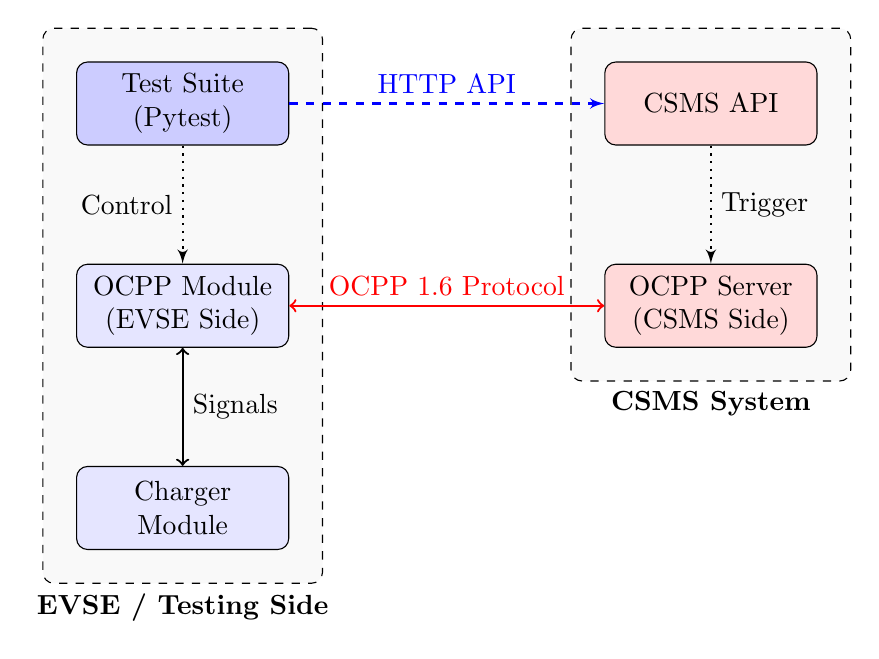
\begin{tikzpicture}[
    node distance=2.5cm,
    block/.style={rectangle, draw, fill=blue!10, text width=7em, text centered, rounded corners, minimum height=3em},
    container/.style={draw, rectangle, dashed, inner sep=1.2em, fill=gray!5, rounded corners},
    line/.style={draw, -latex', thick},
    api/.style={draw, -latex', thick, dashed, color=blue},
    ocpp/.style={draw, -latex', thick, color=red},
    control/.style={draw, -latex', thick, dotted, color=black}
]

    % Layer 1: Entrance / Management Layer
    \node [block, fill=blue!20] (testsuite) {Test Suite (Pytest)};
    \node [block, right=4cm of testsuite, fill=red!15] (csms_api) {CSMS API};
    
    % Layer 2: Communication Layer (Aligned Horizontally)
    \node [block, below=1.5cm of testsuite] (interface) {OCPP Module\\(EVSE Side)};
    \node [block, below=1.5cm of csms_api, fill=red!15] (csms_ocpp) {OCPP Server\\(CSMS Side)};
    
    % Layer 3: System Base / Hardware
    \node [block, below=1.5cm of interface] (charger) {Charger Module};
    
    % Group Containers (on background layer)
    \begin{scope}[on background layer]
        \node [container, fit=(testsuite) (interface) (charger)] (evse_group) {};
        \node [container, fit=(csms_api) (csms_ocpp)] (csms_group) {};
    \end{scope}

    \node [below] at (evse_group.south) {\textbf{EVSE / Testing Side}};
    \node [below] at (csms_group.south) {\textbf{CSMS System}};

    % Connections
    
    % Test Suite Flow
    \path [api] (testsuite) -- node [midway, above] {HTTP API} (csms_api);
    \path [control] (testsuite) -- node [midway, left] {Control} (interface);
    
    % OCPP Peer-to-Peer (Layer 2)
    \path [ocpp, <->] (interface) -- node [midway, above] {OCPP 1.6 Protocol} (csms_ocpp);
    
    % Internal State 
    \path [line, <->] (interface) -- node [midway, right] {Signals} (charger);
    \path [control] (csms_api) -- node [midway, right] {Trigger} (csms_ocpp);

\end{tikzpicture}

\end{document}
